\section{Implementation} \label{6sec:impl}
%   if you have class diagram
% \\ or an image that show parts of your system
% \\ screenshots of part of your code
% \\ explain the main parts of the code
% \\ make a relation between the functionalities of the system and the requirements
% \\ like: this part of the code does that which is described in the requirement FR1.

The following section will explain the general structure of the system,
as well as some important specific aspects of the implementation.
One part of the system is the CARLA simulation,
which represents the central Smart City.


% \begin{figure}[H]
%   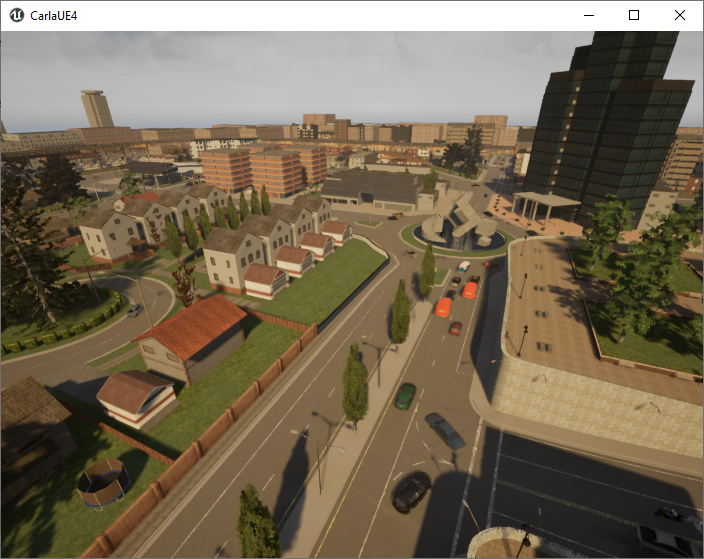
\includegraphics[width=0.6\linewidth]{chapters/chapter6_bruno/Figures/UECity1.png}
%   \caption{City rendered in Unreal Engine 4}
%   \label{6fig:cityRender}
% \end{figure}
\begin{wrapfigure}{r}{0.5\textwidth}
    \vspace{-0pt}
  \centering{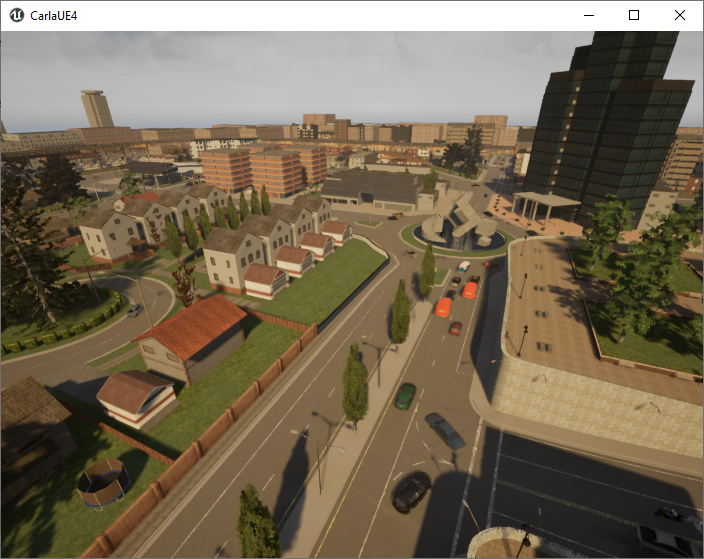
\includegraphics[width=\linewidth]{chapters/chapter6_bruno/Figures/UECity1.png}}
    \vspace{-10pt}
  \caption{City rendered in Unreal Engine 4}
  \label{6fig:cityRender}
    \vspace{-10pt}
\end{wrapfigure}

\noindent
This simulation runs independently of the rest of the project
and is also not part of the source code in this projects GitHub repository.

\noindent
It could be hosted on any cloud,
although for all tests of the project
it was running on the same PC as the crash-detection program.
\\
\newline
The simulation is running on the Unreal Engine 4 
and looks like Figure \ref{6fig:cityRender} while its online.
In this window, a flying camera can be controlled,
to watch over the city,
but a no-render mode is also available for the simulation.
There are a few different cities to load in already in CARLA,
but custom levels could also be generated.
After the crash-detection program has connected to the simulation,
in the case of the tests to the localhost,
it can intact with the simulation through the Python API from CARLA. 
\\
\newline
The starting point for the rest of the system is the \emph{main.py} file.
Here basics like ensuring the right
working directory or the command-line arguments are set up.

\begin{wrapfigure}{l}{0.4\textwidth}
    \vspace{-16pt}
  \centering{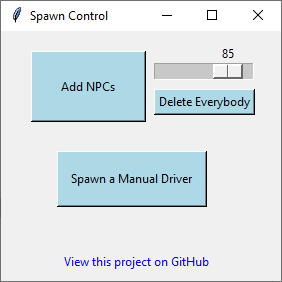
\includegraphics[width=\linewidth]{chapters/chapter6_bruno/Figures/ui1.png}}
    \vspace{-10pt}
  \caption{Tkinter window}
  \label{6fig:ui}
    \vspace{-10pt}
\end{wrapfigure}

\noindent
After that, the window seen in Figure \ref{6fig:ui} is initialised.
For this, the package Tkinter was used.
This is the center for all action from the user.
They can add an adjustable number of NPCs to the simulation or delete all of them. 
These will drive autonomously around the town, as can be seen in Figure \ref{6fig:cityRender}.
They serve mostly as obstacles to crash into and have no further functionality to them.

\noindent
The process of actually spawning the cars into the simulation
is handled by one of the example scripts from the Python API,
\emph{spawn\_npc.py}.
\\
\newline
The framework for the manual driver is also mostly 
from the example script \emph{manual\_control.py}.
The following section will still though go over the basic principle behind it
and then explain when new features were added for this project.

\subsection{Manual Driver}\label{6sec:manCar}
\noindent
When the \emph{Spawn a Manual Driver} Button in Figure \ref{6fig:ui} is pressed,
a new thread is started, using the multiprocessing package.
This thread then executes the above mentioned script.
Using threading means that the user can generate as many manual drivers as they want,
only being limited by their system resources.

\noindent
At the start of the script,
a connection to the MQTT server was added.
The each manual car is given a random name from a list 
and a random ID to identify them. 
This driver is then registered on the server,
with a message with an empty reason and all information on the driver.

\noindent
After that the heart monitor was added.
It is started as a new thread, always running in the background 
of every active manual car. 
As a simulation of a real pulse sensor,
it generates a random number of a normal curve every second.

Then the code of the example script is executed. 
It first connects to the simulation,
which was running on the localhost for all tests.
Then a drivable car is created, via the "blueprints" provided by CARLA.
This car then gets sensors attached, also from blueprints.
In a final loop the window depicted in Figure \ref{6fig:manCar} is rendered,
with a few HUD elements and a camera following the car. 
The user can now control the car using the arrow-keys on the keyboard.

\begin{figure}[H]
  \centering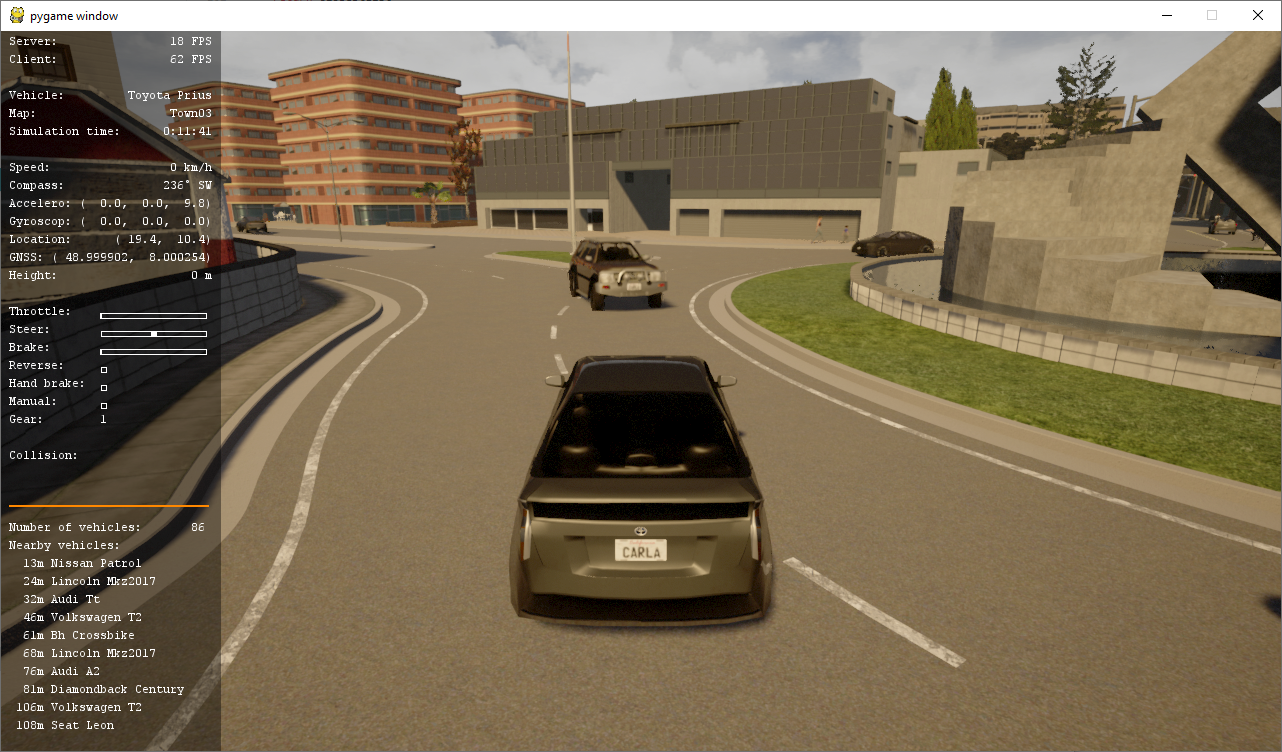
\includegraphics[width=0.9\linewidth]{chapters/chapter6_bruno/Figures/manual1.png}
  \caption{Manually Controllable Car}
  \label{6fig:manCar}
\end{figure}

\noindent
As mentioned, these cars have a collision sensor.
This sensor is continually listening to a \emph{\_oncollision\_()} method. 
This made it very easy to implement the concept of monitoring crashes.

\begin{wrapfigure}{l}{0.55\textwidth}
    \vspace{-16pt}
  \centering{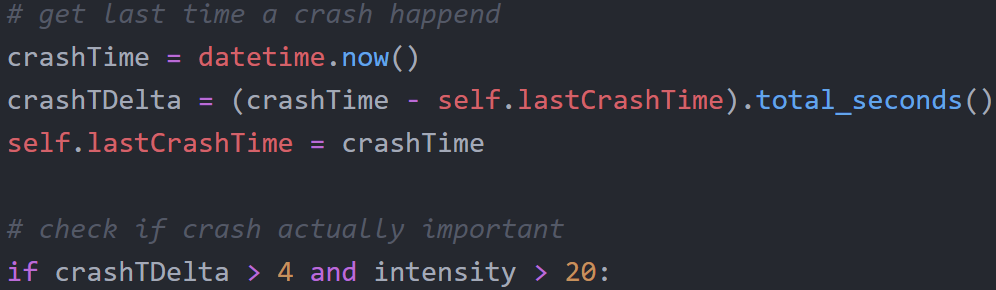
\includegraphics[width=\linewidth]{chapters/chapter6_bruno/Figures/collisionCode.png}}
    \vspace{-16pt}
  \caption{Time and force filter}
  \label{6fig:onCollCode}
    \vspace{-18pt}
\end{wrapfigure}

\noindent
First a filter was added, seen in Figure \ref{6fig:onCollCode},
which checks the validity of the crash.
The timestamp of the crash is compared to the one of the last registered crash.
Then, if the this last crash didn't happen in the last 4 seconds
and if the intensity of the collision is high enough,
the emergency message will be generated (Figure \ref{6fig:onCollCode2}).

\noindent
This filter ensures two things.
A single car crash could consist of multiple impacts in quick succession,
which would otherwise all activate their own messages.
It also removes false positives, from small impacts
like a speed bump.
\begin{wrapfigure}{l}{0.55\textwidth}
    \vspace{-6pt}
  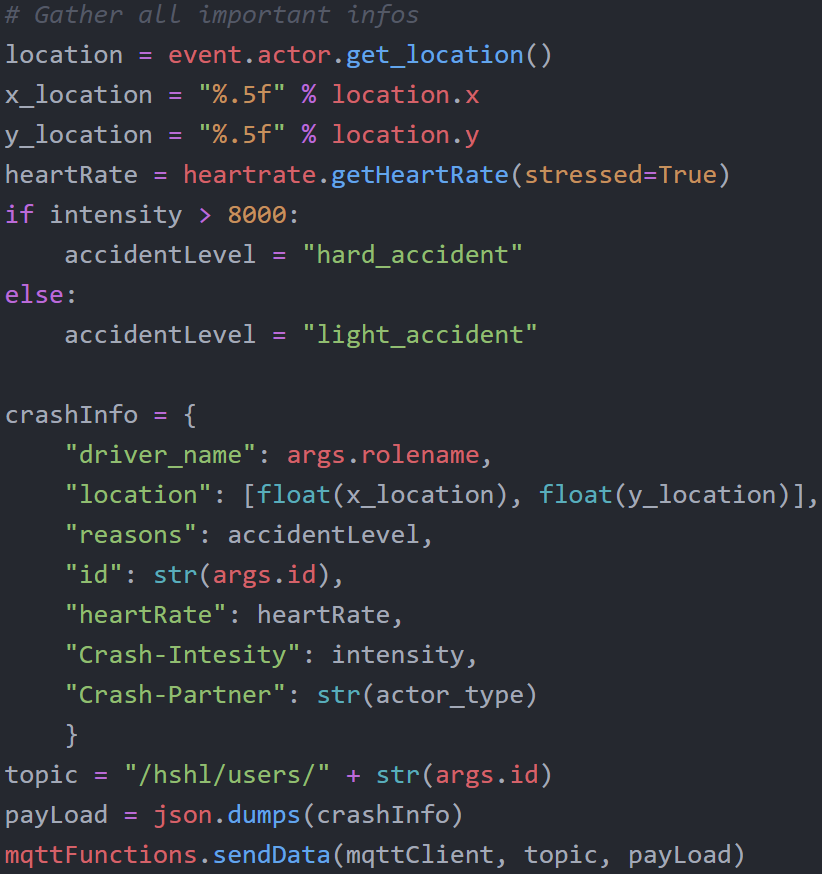
\includegraphics[width=\linewidth]{chapters/chapter6_bruno/Figures/collisionCode2.png}
    \vspace{-10pt}
  \caption{Message Generation}
  \label{6fig:onCollCode2}
  \vspace{-20pt}
\end{wrapfigure}
\\
\noindent
If the crash is validated, additional information on the crash is gathered,
as can be seen at the top of Figure \ref{6fig:onCollCode2}.
Its also decided whether to classify the crash as a hard or a light one,
which could potentially change the reaction from the server.
\\
\newline
Finally, all relevant information gets stored as a json dump,
which converts them into a long string that is compatible with the MQTT protocol.
The message is then send to the specific topic of the driver.\linebreak

\noindent
After that the system the checks if the heart rate of the driver is critical.
If so, a second, slightly different message will be created and send.
It only contains the basic driver information and
is intended to be forwarded to the ambulances of the city.

\noindent
This is done to fulfill the requirements G2.2 and G2.3.
Those were created when the concept of the server wasn't final yet
and were intended for a slightly different message handling structure.
This system is still fully functional,
but the second message is not really needed today.
